\section{Numerical experiment}
We design two numerical experiments to illustrate that msTVGL is able to alleviate heterogeneity between subjects when sample sizes are unequal, 
and to avoid imbalanced sparsity penalty of precision matrices due to uneven sample sizes across all time points.
The measures of criterion across the two experiments are F1-score and temporal deviation ratio, 
where F1-score illustrates the accuracy of edge recovery and temporal deviation ratio shows whether the algorithm catches the correct time-varying dynamic of precision matrices or not. 
The F1-score is the harmonic mean of the precision and recall: $\frac{2*\text{precision}*\text{recall}}{\text{precision} + \text{recall}}$, 
where $\text{precision}:=\frac{\text{TP}}{\text{TP} + \text{FP}}$ and $\text{recall}:=\frac{\text{TP}}{\text{TP} + \text{FN}}$.
It balances the weights of precision and recall, 
and is suitable for scenarios where the importance of both is comparable.

\subsection{Test 1: Accuracy on network recovery}
We show that the average within-subject sample covariance matrix contributes to the robustness on the network recovery 
when heterogeneity between subjects exists and sample sizes of isolated subjects outnumber the ones of integrated subjects. 
However, in the opposite situation, the TVGL method outperforms the msTVGL. 
Moreover, when sample sizes of all subjects are almost equal, 
the average within-subject sample covariance matrix is equivalent to the scaled sample covariance matrix of all mixed observations, 
thereby won't bring additional robustness.

In this experiment, 
a series of smooth varying random symmetric positive definite matrices are chosen as the ground truth precision matrices $\Theta_1,\cdots,\Theta_T$. 
Only precision matrix entries larger than 0.05 are recognized as valid edges and vise versa. 
We equally assign 10 subjects for all time points.  
At time point $t_i$, there are $(1-p)\times100\%$ of subjects following the Gaussian distribution $\mathcal{N}(0,\Theta_i^{-1})$ and 
$p\times100\%$ of subjects containing samples from a Gaussian distribution $\mathcal{N}(0,\Theta_{i,noise}^{-1})$ with a noise precision matrix $\Theta_{i,noise}$ exactly different from $\Theta_i$. 
We call $p\in[0,1]$ the abnormality fraction and test it with $0, 0.1, 0.2, 0.3, 0.4, 0.5$ in the numerical experiment. 
For each value of $p$, we run msTVGL and TVGL with Laplacian temporal penalty for 10 times, 
and for each turn a dataset generated as aforementioned are used by the two methods.
Then we calculate the mean of F1-score at each time point and the mean of temporal deviation ratio. 
The hyperparameters are respectively set for msTVGL and TVGL to keep the average F1-score across all time points above 0.9 when $p=0$. 
For msTVGL, we set $\lambda=0.001$ and $\beta=0.01$, 
while for TVGL $\lambda=0.35$ and $\beta=0.01$. 

To test the three case when i) subjects with the most observations are more heterogeneous than others; 
ii) subjects with the least observations are more heterogeneous than others; 
iii) all subjects have almost equal sample size,
we consistently set sample sizes of 10 subjects across all time points by $[2000, 1600, 1200, 1500, 1100, 500, 450, 400, 550, 500]$, 
$[500, 450, 400, 550, 500, 2000, 1600, 1200, 1500, 1100]$ and $[1500, 1450, 1400, 1550, 1500, 2000, 1600, 1200, 1500, 1100]$ 
respectively. 
As abnormality fraction $p$ goes from 0.1 to 0.5, 
the first 1 to 5 subjects gain heterogeneity by using noise precision matrix $\Theta_{i,noise}$ 
to generate samples. 

The results for cases i), ii) and iii) are shown in Figure \ref{fig: Num_isolated_larger_integrated_F1}
to \ref{fig: Num_isolated_equals_integrated_TDR}.

The result can be roughly explained by trace term of the loss function in both msTVGL and TVGL. 
Suppose at time $t_i$, there are in total $n_i$ samples for $N_i$ subjects, 
with $n_i=\sum_{k=1}^{N_i}n_{ik}$. 
When related to $\Theta_i$, 
the trace term of msTVGL negative log-likelihood loss is given by 
\begin{equation*}
    \text{Tr}(\sum_{k=1}^{N_i}S_{ik}\Theta_i) = \sum_{k=1}^{N_i}\text{Tr}(S_{ik}\Theta_i) 
    = \sum_{k=1}^{N_i}\frac{1}{n_{ik}}\text{Tr}(\sum_{j=1}^{n_{ik}}x_jx_j^T\Theta_i). 
\end{equation*}
The trace term of TVGL negative log-likelihood loss (up to a scale $n_i$) is given by 
\begin{equation*}
    \text{Tr}(S_i\Theta_i) = \text{Tr}(\frac{1}{n_i}\sum_{j=1}^{n_i}x_jx_j^T\Theta_i)
    = \sum_{k=1}^{N_i}\frac{1}{n_i}\text{Tr}(\sum_{j=1}^{n_{ik}}x_jx_j^T\Theta_i). 
\end{equation*}

When relatively isolated subjects and the integrated ones don't have equal samples, 
we focus on the trace term of TVGL negative log-likelihood. 
\begin{equation*}
    \text{Tr}(S_i\Theta_i) = \sum_{k=1}^{N_i}\text{Tr}(\frac{1}{n_i}\sum_{j=1}^{n_{ik}}x_jx_j^T\Theta_i) 
    = \text{Tr}(\sum_{k=1}^{N_i}\tilde{S}_{ik}\Theta_i), 
\end{equation*}
where $\tilde{S}_{ik}=\frac{n_{ik}}{n_i}S_{ik}$. 
It is clear that $\tilde{S}_{ik}$ is close to the sample covariance matrix $S_{ik}$ if $n_{ik}$ is large, 
and deviate from it otherwise. 
Hence, $\sum_{k=1}^{N_i}\tilde{S}_{ik}$ is composed by the the sum of the slightly deviated sample covariance matrices for subjects with large sample sizes, 
and the sum of the heavily deviated sample covariance matrices for subjects with small sample sizes. 
Consequently, the estimated precision matrix from TVGL incorporates more information from observations corresponding to subjects with large sample sizes.
Since msTVGL equally treat the sample covariance matrices, 
the precision matrix it estimates only depends on the accuracy of sample covariance matrix to the true covariance matrix 
without any weights further amplifying the inequality on the sample size.

When $n_{i1}\approx\cdots\approx n_{iN_i}$, 
we have that 
\begin{equation*}
    \text{Tr}(S_i\Theta_i) = \text{Tr}(\sum_{k=1}^{N_i}\tilde{S}_{ik}\Theta_i)
    = \text{Tr}(\sum_{k=1}^{N_i}\frac{n_{ik}}{n_i}S_{ik}\Theta_i)
    \approx \frac{1}{N_i}\text{Tr}(\sum_{k=1}^{N_i}S_{ik}\Theta_i),  
\end{equation*}
which means the negative log-likelihood loss of TVGL (\ref{eq: ch1_loss_paper}) is around $\frac{n_i}{N_i}$ times of the one of msTVGL (\ref{eq: ch1_loss_modify1_normalized}). 
This explains the similar performance of the two methods when all subjects have almost equal sample size for all time points. 

\subsection{Test 2: Avoiding imbalanced sparsity penalty}
We show the loss function of msTVGL avoids imbalanced sparsity penalty caused by uneven total sample sizes across all time points. 

In this experiment, 
the precision matrices across all time points are stationary, i.e. $\Theta_1=\cdots=\Theta_T$.
Only precision matrix entries larger than 0.05 are recognized as valid edges and vise versa. 
We equally assign 10 subjects for all time points. 
At time point $t_i$, all subjects consistently follow the Gaussian distribution $\mathcal{N}(0,\Theta_i)$. 
To clearly display the imbalanced sparsity penalty, 
we abandon the temporal smoothness penalty by setting $\beta=0$,
and impose large gap between the largest and the smallest sample sizes. 
The sample sizes across all time points descend from 2000 to 250 and then rise from 250 to 2000. 
We iteratively run msTVGL and TVGL on the same observations by looping spatial penalty parameter $\lambda$ within sets 
$[0.1, 0.2, 0.3, 0.4, 0.5, 10]$ and $[10, 50, 100, 150, 200, 250]$ respectively. 
Then we calculate the mean of F1-score at each time point and the mean of temporal deviation ratio. 

The results is shown in Figure \ref{fig: Num_imbalanced_F1} and \ref{fig: Num_imbalanced_TDR}.
An intuitive mathematical explanation has already been provided in Subsection \ref{subsec: hyperparameters}. 

\subsection{Result images}

\begin{figure}[htbp]
    \centering
    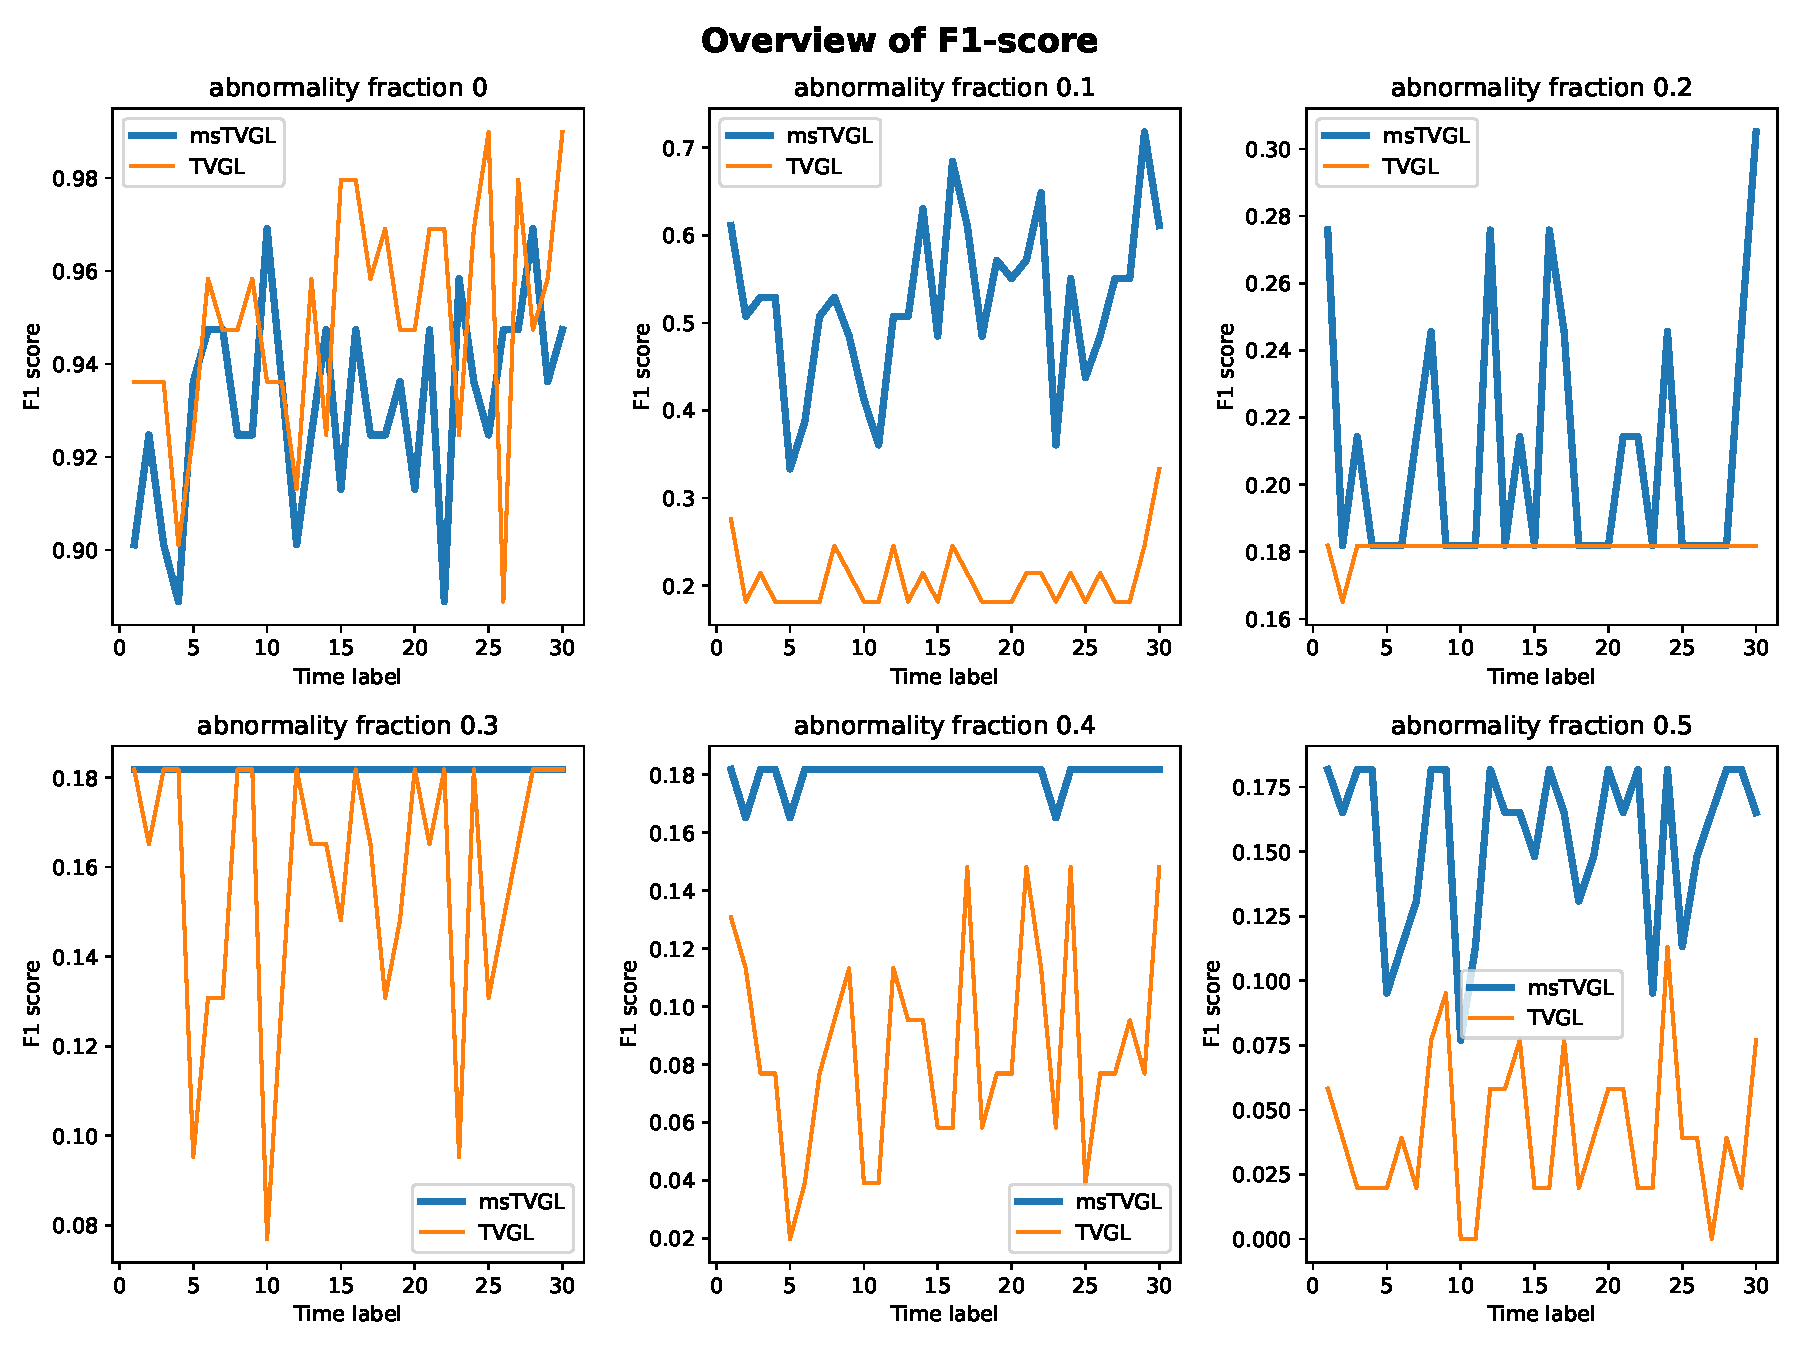
\includegraphics[width=\textwidth]{images/isolated_larger_integrated_F1.pdf}
    \caption{\centering The F1-score for case i).}
    \label{fig: Num_isolated_larger_integrated_F1}
\end{figure}

\begin{figure}[htbp]
    \centering
    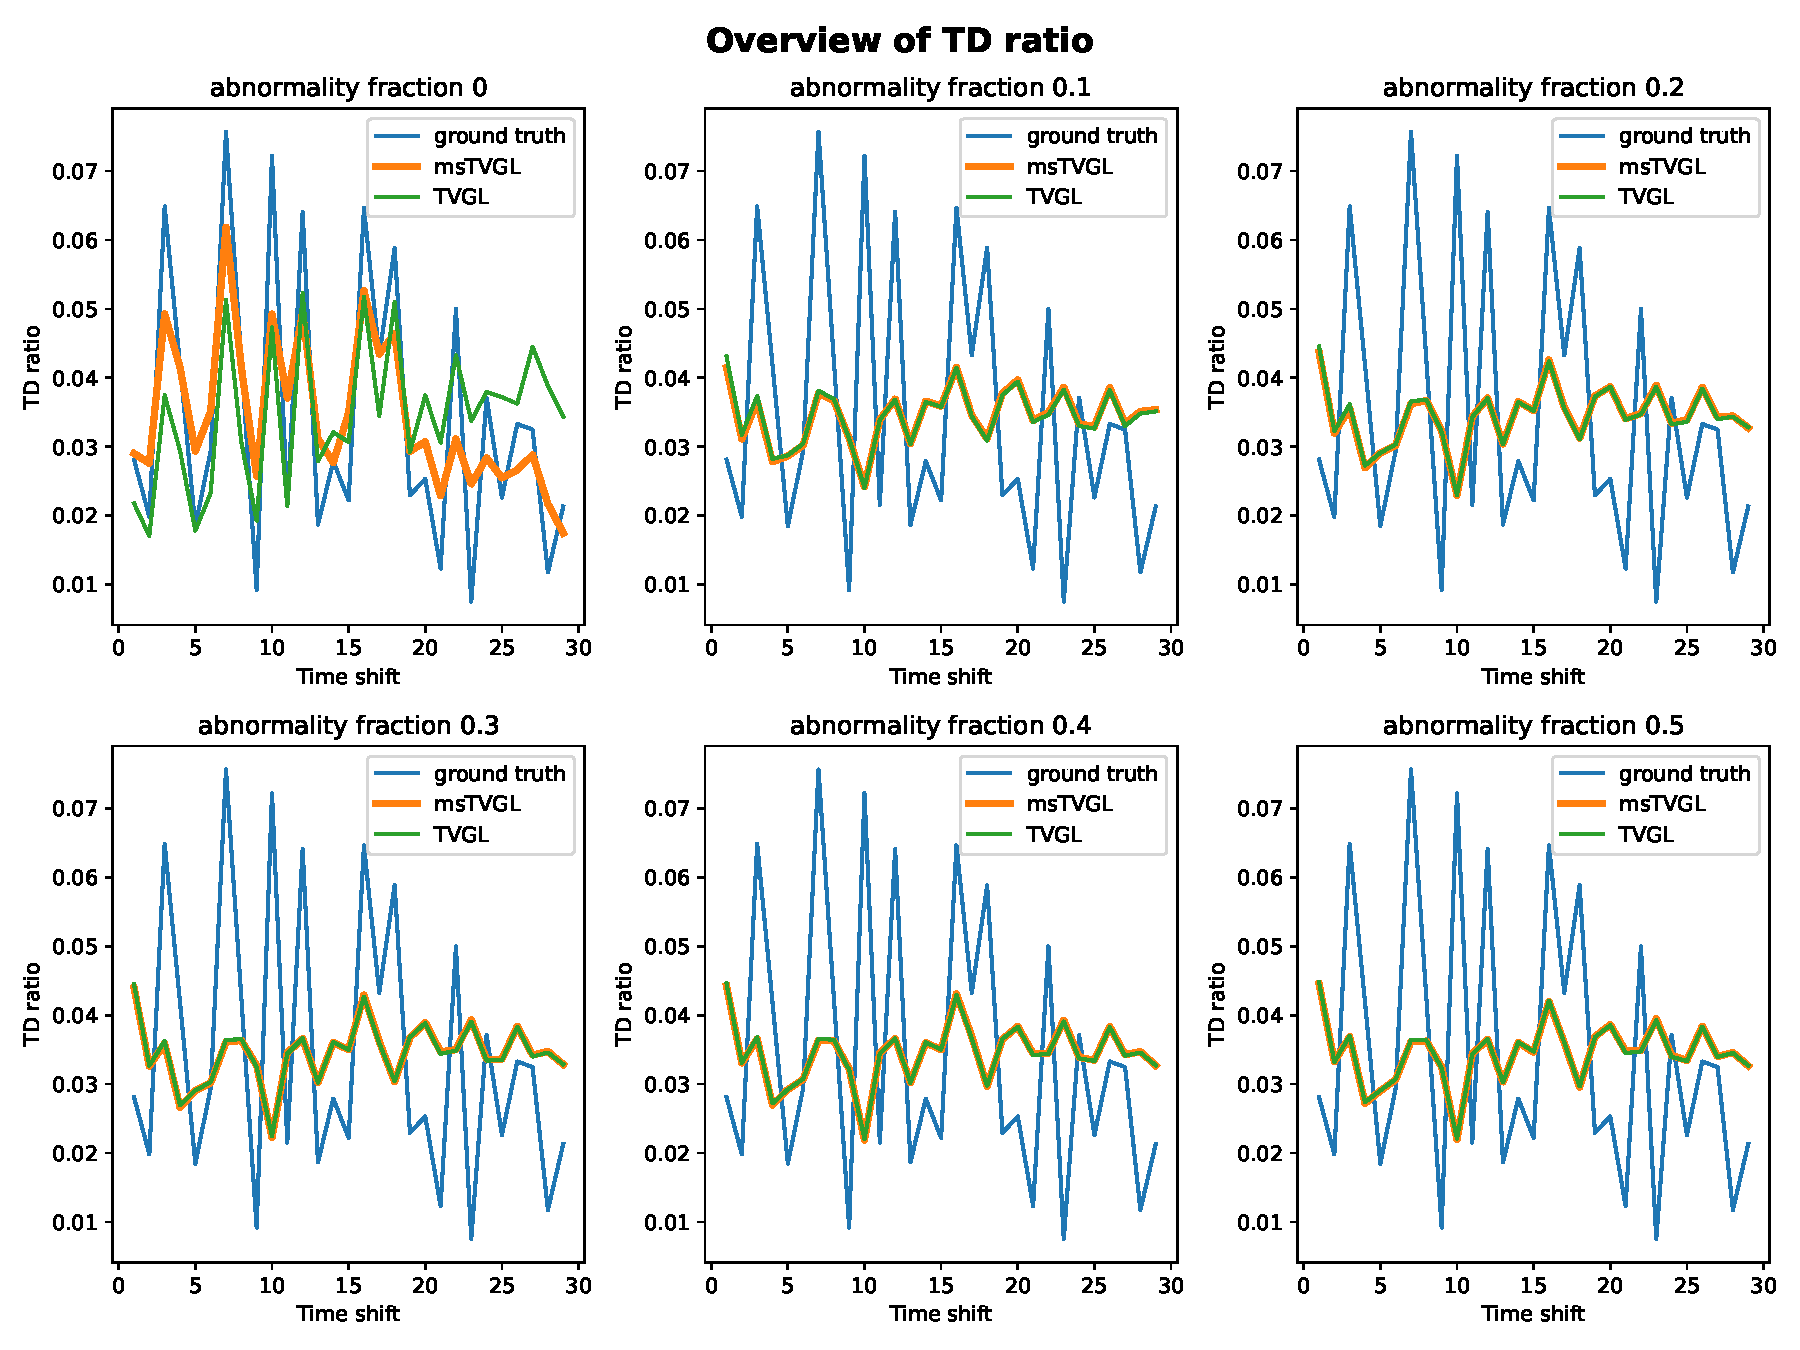
\includegraphics[width=\textwidth]{images/isolated_larger_integrated_TDR.pdf}
    \caption{\centering The temporal deviation ratio for case i).}
    \label{fig: Num_isolated_larger_integrated_TDR}    
\end{figure}

\begin{figure}[htbp]
    \centering
    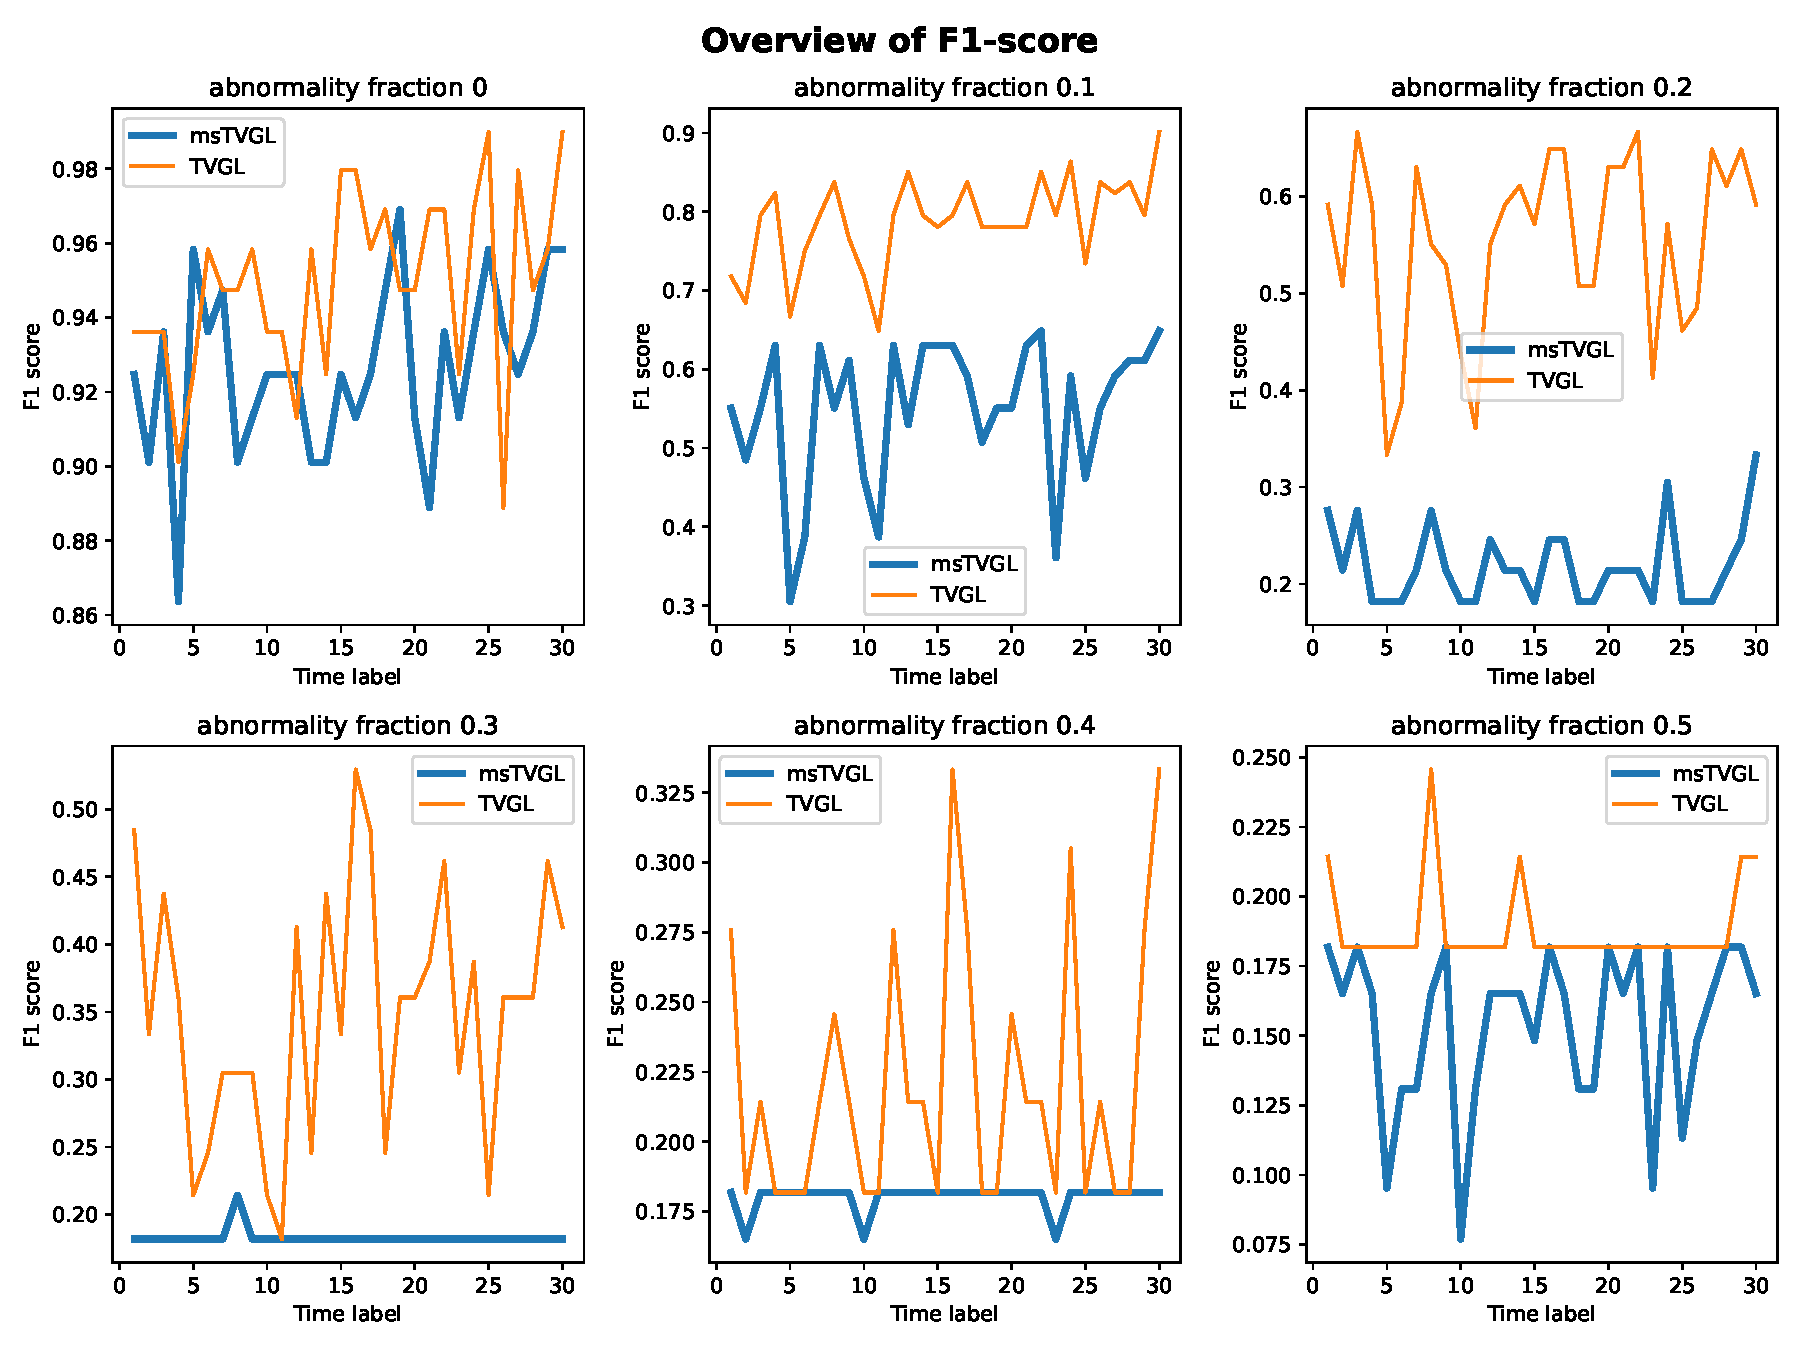
\includegraphics[width=\textwidth]{images/isolated_smaller_integrated_F1.pdf}
    \caption{\centering The F1-score for case ii).}
    \label{fig: Num_isolated_smaller_integrated_F1}
\end{figure}

\begin{figure}[htbp]
    \centering
    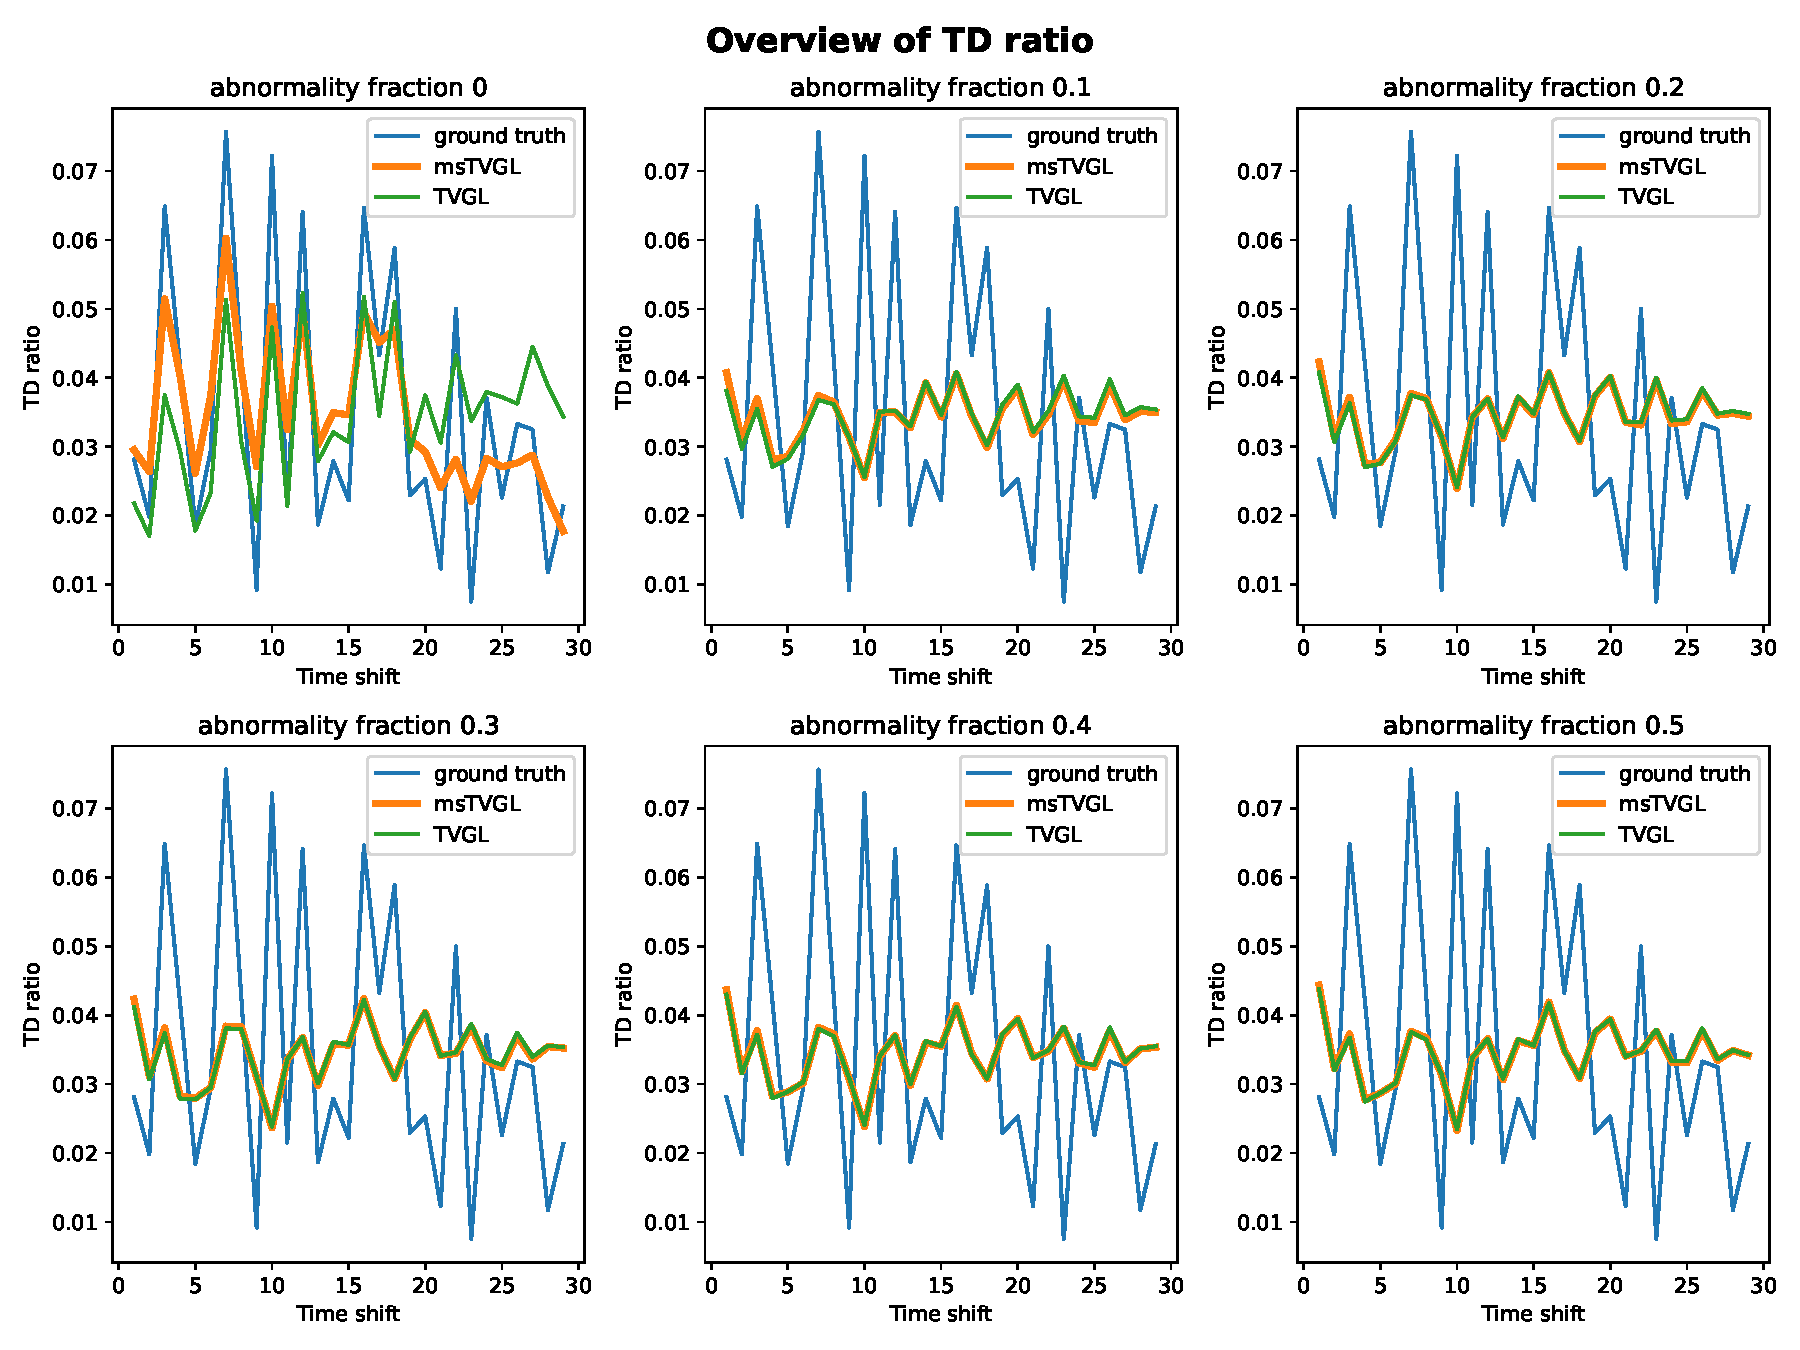
\includegraphics[width=\textwidth]{images/isolated_smaller_integrated_TDR.pdf}
    \caption{\centering The temporal deviation ratio for case ii).}
    \label{fig: Num_isolated_smaller_integrated_TDR}    
\end{figure}

\begin{figure}[htbp]
    \centering
    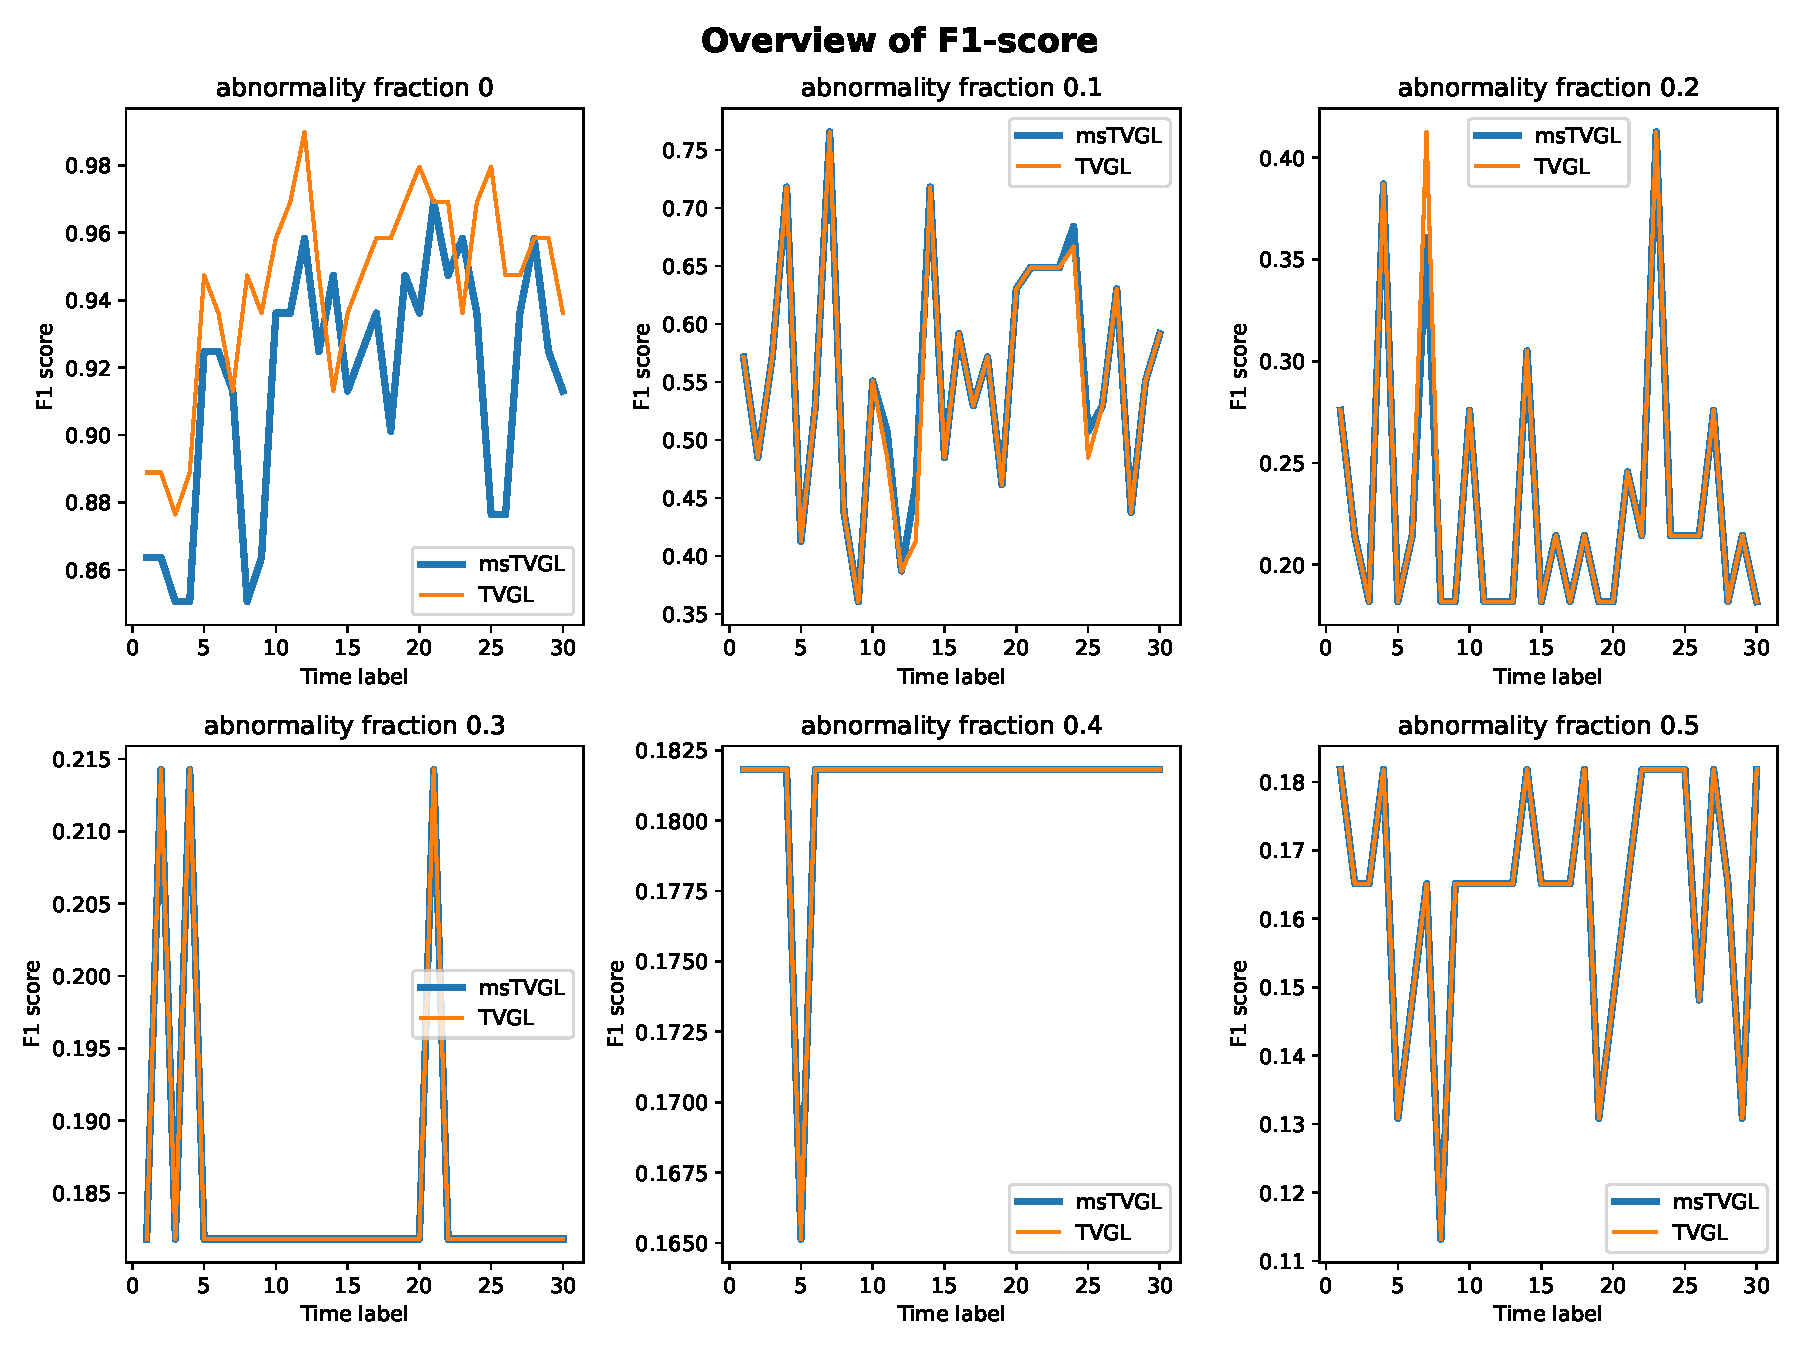
\includegraphics[width=\textwidth]{images/isolated_equals_integrated_F1.pdf}
    \caption{\centering The F1-score for case iii).}
    \label{fig: Num_isolated_equals_integrated_F1}
\end{figure}

\begin{figure}[htbp]
    \centering
    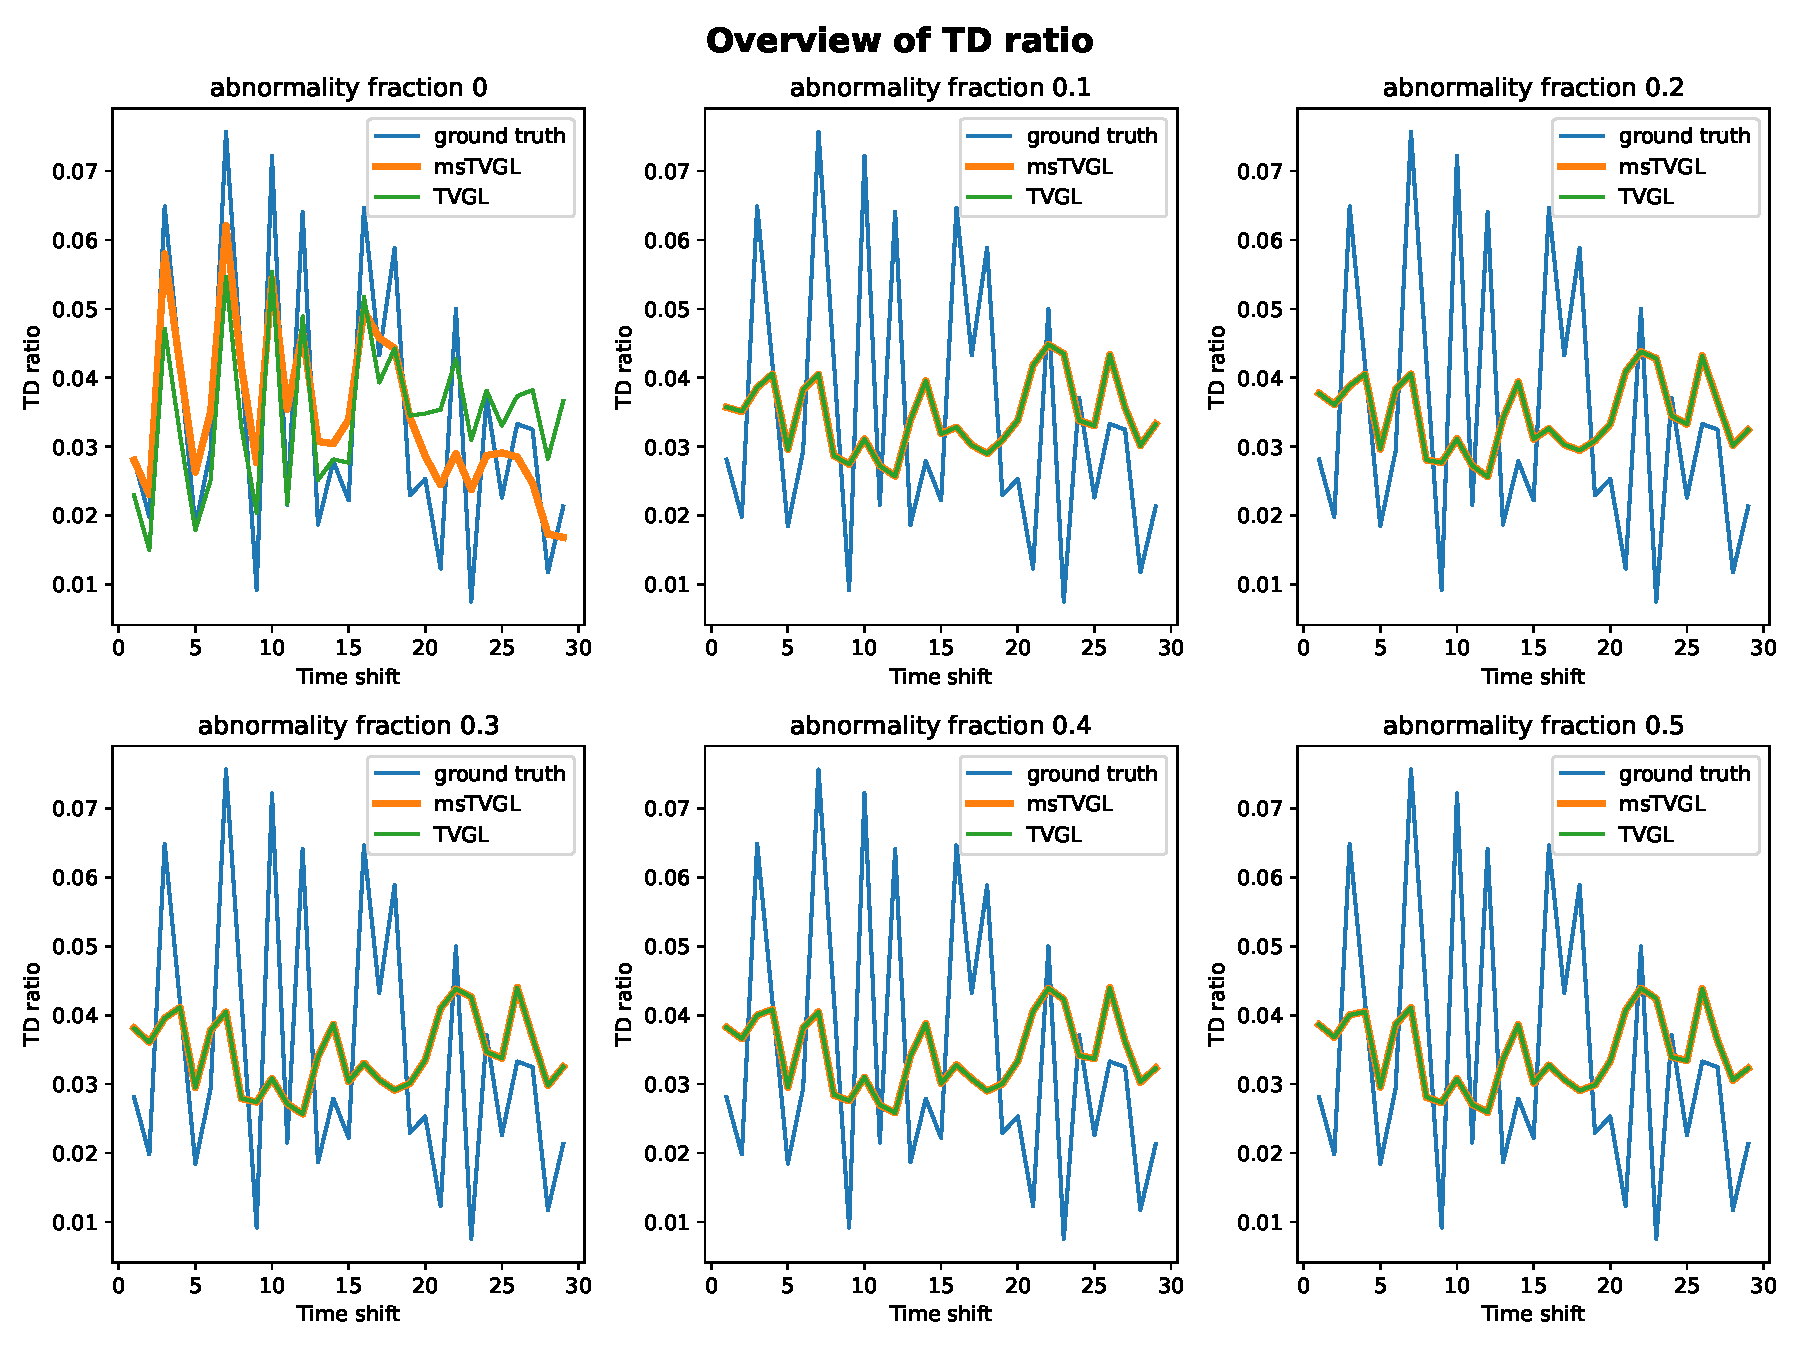
\includegraphics[width=\textwidth]{images/isolated_equals_integrated_TDR.pdf}
    \caption{\centering The temporal deviation ratio for case iii).}
    \label{fig: Num_isolated_equals_integrated_TDR}    
\end{figure}

\begin{figure}[htbp]
    \centering
    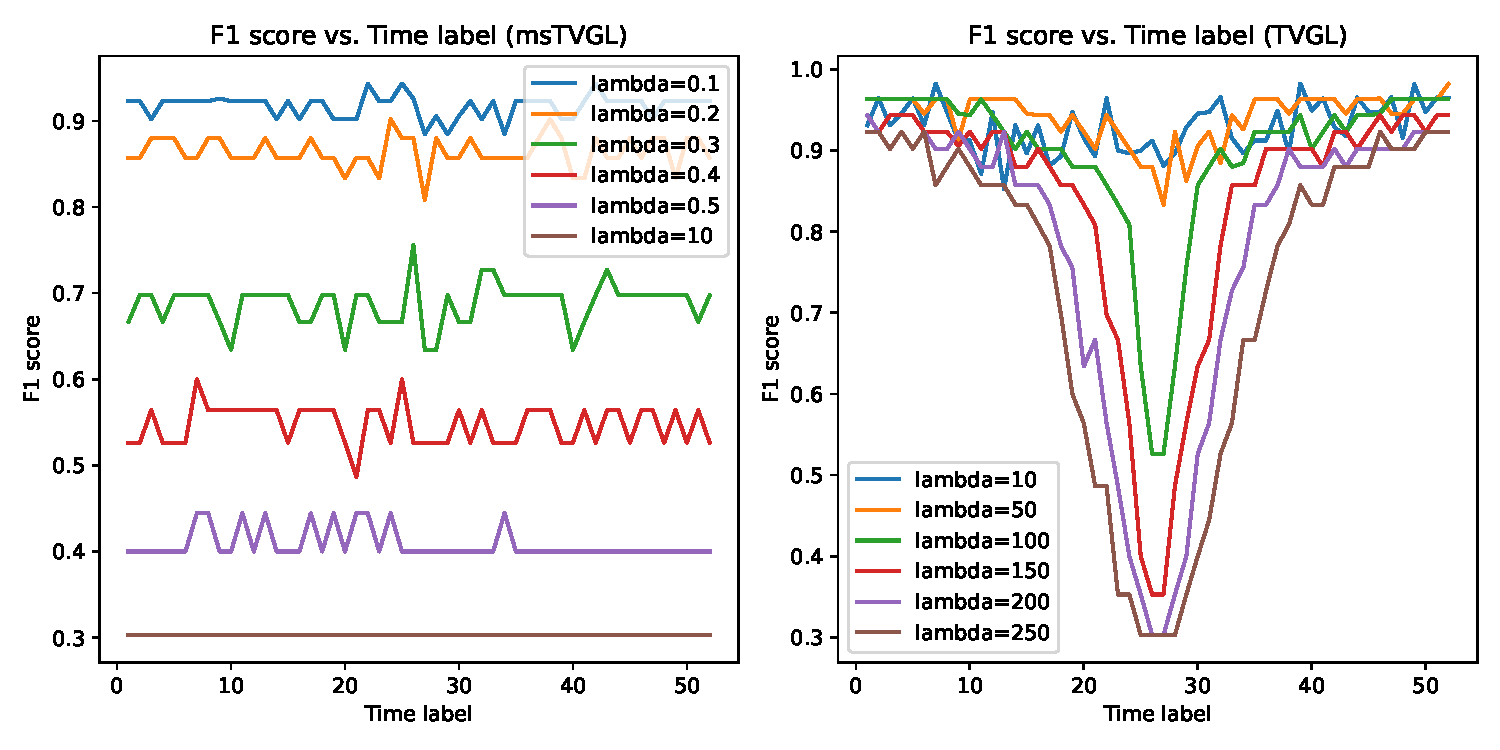
\includegraphics[width=\textwidth]{images/Imbalanced_F1.pdf}
    \caption{\centering The F1-score for test on imbalanced sparsity penalty.}
    \label{fig: Num_imbalanced_F1}
\end{figure}

\begin{figure}[htbp]
    \centering
    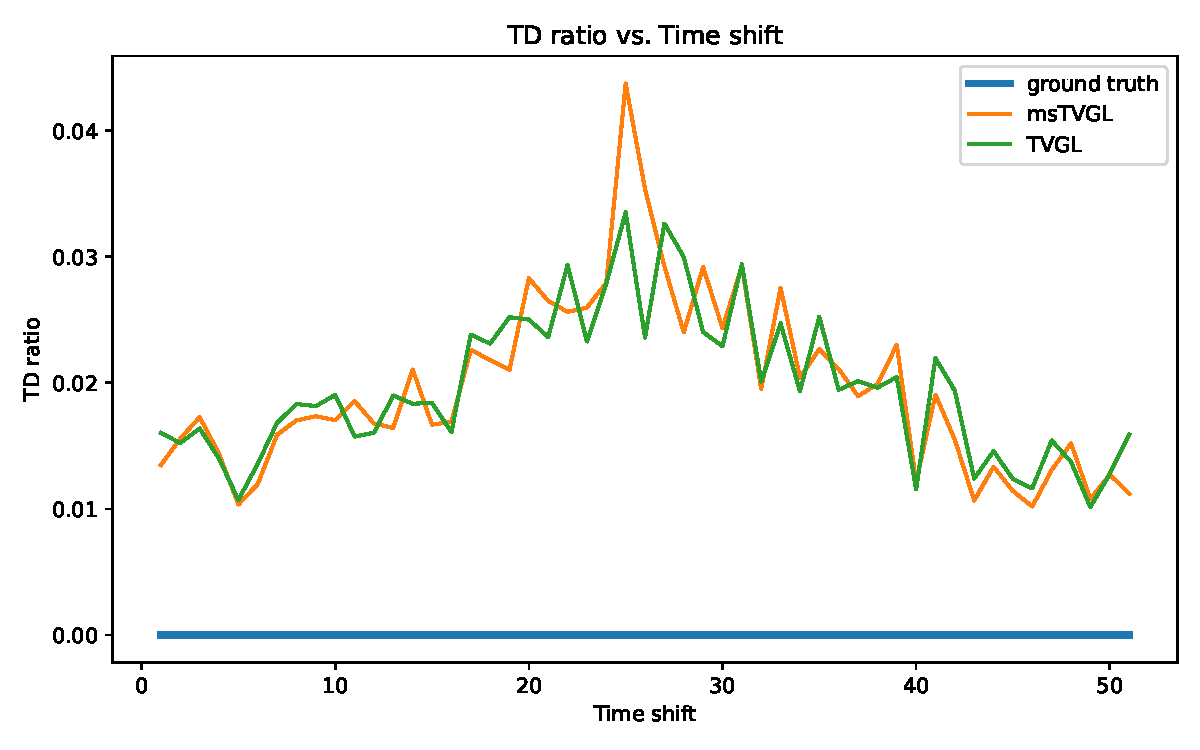
\includegraphics[width=\textwidth]{images/Imbalanced_TDR.pdf}
    \caption{\centering The temporal deviation ratio for test on imbalanced sparsity penalty.}
    \label{fig: Num_imbalanced_TDR}
\end{figure}